\RequirePackage{atbegshi} % Background stuff below trim marks
\AtBeginShipoutInit
\documentclass[avery5371]{flashcards}

%%% PACKAGES
\usepackage{changepage} % page check
\strictpagecheck
\usepackage{amssymb} % boxes
\usepackage{amsmath} % maths
\usepackage{lipsum} % dummy text
\usepackage{ragged2e} % switch commands to flushLeft/right
\usepackage{graphicx} % include jged, png, etc.
\graphicspath{{./images/}} 
\usepackage[export]{adjustbox} % use adjustbox keys in includegraphics, e.g. max height/width
\usepackage{svg} % include svg using inkscape
\usepackage[top]{background} % Background stuff
\usepackage{eso-pic} % AddToShipoutPictureBG
\usepackage{tikz} % tikz drawing
\usepackage{xcolor} % custom colors
\definecolor{uniscielblue}{RGB}{4,146,191}
\definecolor{uniscielpink}{RGB}{231,33,90}
\definecolor{uniscielgrey}{RGB}{103,104,104}
\definecolor{physicsviolet}{HTML}{463374}
% Bleu : #0492bf
% Rose : #e7215a
% Gris : #676868
% Violet : #463374

%%% FONTS %%%%
\usepackage{fontspec}
\setsansfont{Eufoniem One}

%%% GEOMETRY AND BLEED MARKS %%%
\geometry{
    papersize = {100 truemm, 80 truemm},
    margin = 0 truemm
    % marginparwidth = 0 truemm,
    % marginparsep = 0 truemm
}
\usepackage[
width = 110 truemm,
height = 90 truemm,
frame,
cam,
noinfo,
center,
]{crop}    


%%% FLASHCARDS PARAMETERS %%%
% Card size and margins
\renewcommand{\cardpapermode}{portrait}
\renewcommand{\cardrows}{1}
\renewcommand{\cardcolumns}{1}
\setlength{\cardwidth}{9.7 cm}
\setlength{\cardheight}{7.5 cm}

\setlength{\cardmargin}{2 mm}
\setlength{\topoffset}{0 mm}
\setlength{\oddoffset}{0 mm}
\setlength{\evenoffset}{0 mm}

% Card Background
\SetBgScale{1.0}                          % Select scale factor
\SetBgAngle{0.0}                          % Select rotation
% \SetBgOpacity{0.5}                        % Select opacity
% \SetBgContents{\bgimage{0.15}{0.8}}       % Set tikz picture
% \SetBgPosition{current page.north west}   % Select location

% Card styles and fonts
\cardfrontstyle[\footnotesize]{plain}
\cardbackstyle[\footnotesize]{plain}

%%% CUSTOM COMMANDS %%%

\newcommand{\backgroundparam}[8]{
    \providecommand{\subjecticon}{#1}
    \providecommand{\frontheader}{#2}
    \providecommand{\frontfooter}{#3}
    \providecommand{\backbackground}{#4}
    \providecommand{\backheader}{#5}
    \providecommand{\backfooter}{#6}
    \providecommand{\frontuniversitylogo}{#7}
    \providecommand{\backuniversitylogo}{#8}
    \renewcommand{\subjecticon}{#1}
    \renewcommand{\frontheader}{#2}
    \renewcommand{\frontfooter}{#3}
    \renewcommand{\backbackground}{#4}
    \renewcommand{\backheader}{#5}
    \renewcommand{\backfooter}{#6}
    \renewcommand{\frontuniversitylogo}{#7}
    \renewcommand{\backuniversitylogo}{#8}
}

\newcommand{\cardbackground}[4]{
    \SetBgContents{
        \AddToShipoutPictureBG*{    
            \begin{tikzpicture}[remember picture, overlay]
                \checkoddpage
                \ifoddpage
                    % Subject front header
                    \node at ([xshift = -0.85 cm, yshift = -0.85 cm]current page.north) {
                        \includesvg[width = 0.9\textwidth]{\frontheader}
                    };
                    % Subject front footer
                    \node at ([xshift = 0.75 cm, yshift = 0.5 cm]current page.south) {
                        \includesvg[width = 0.9\textwidth]{\frontfooter}
                    };
                    % Subject icon
                    \node [opacity = 1] at ([xshift = 1.25 cm, yshift = -1 cm]current page.north west) {
                        \includesvg[height = 0.175\textheight]{icons/\subjecticon}
                    };
                    % Subject text
                    \node [opacity = 1] at ([xshift = -1.4 cm, yshift = -0.75 cm]current page.north) {
                        \color{white}
                        \huge
                        \textsf{#2}
                    };
                    % Theme
                    \node [opacity = 1] at ([xshift = 2.25 cm, yshift = -2 cm]current page.north) {
                        \begin{varwidth}{0.5\textwidth}
                            \setlength{\parskip}{0 cm}
                            \color{uniscielblue}
                            \RaggedLeft
                            \LARGE
                            \textsf{#3}    
                        \end{varwidth}
                    };
                    % University front logo
                    \node [opacity=1] at ([xshift = -1.75 cm, yshift = 0.75 cm]current page.south east) {                    
                        \includegraphics[max height = 0.135\textheight, center, keepaspectratio]{\frontuniversitylogo}
                    };
                    % Complexity level
                    \node [opacity=1] at ([xshift = -2.75 cm, yshift = 1.175 cm]current page.south) {
                        \color{uniscielpink}
                        \textit{#1}
                    };
                \else
                    % Back background
                    \node at (current page.center) {
                        \includesvg[width = 1.1\textwidth]{\backbackground}
                    };
                    % Subject back header
                    \node at ([xshift = -0.85 cm, yshift = -0.85 cm]current page.north) {
                        \includesvg[width = 0.9\textwidth]{\backheader}
                    };
                    % Subject back footer
                    \node at ([xshift = 0.75 cm, yshift = 0.5 cm]current page.south) {
                        \includesvg[width = 0.9\textwidth]{\backfooter}
                    };
                    % Subject text
                    \node [opacity = 1] at ([xshift = -1.4 cm, yshift = -0.75 cm]current page.north) {
                        \color{physicsviolet}
                        \huge
                        \textsf{#2}
                    };
                    % QR Code
                    \node at ([xshift = 1.375 cm, yshift = -0.85 cm]current page.north west) {
                        \includegraphics[width = 0.150\textwidth, keepaspectratio]{#4}
                    };
                    % University back logo
                    \node [opacity=1] at ([xshift = -1.75 cm, yshift = 0.75 cm]current page.south east) {                    
                        \includesvg[height = 0.135\textheight]{\backuniversitylogo}
                    };
                \fi
            \end{tikzpicture}
        }           
    }
}
\begin{document}
    

\backgroundparam
{physique} % subject icon
{physics-front-header}% Front header filename
{physics-front-footer}% Front footer filename
{physics-back-background}% Back background filename
{physics-back-header}% Back header filename
{physics-back-footer}% Back footer filename
{front_university_logo}% Front university logo
{back_university_logo}% Back university logo

%%%%%%%%%%%%%%% STANDARD TEMPLATE %%%%%%%%%%%%%%%%
\cardbackground
{Niveau de complexité}% Complexity level
{Physique}% Subject
{Lois de Kepler et Newton et leurs applications}% Theme
{qrcode}% qrcode path

\begin{flashcard}[]{
%%% QUESTION %%% 
\color{black}
\vspace{0.15\textheight}
\RaggedRight
% Topic
\'Enoncé\'Enoncé
% Choices
\begin{enumerate}
    \item Réponse 1
    \item Réponse 2 
    \item Réponse 3
    \item Réponse 4
\end{enumerate}
}
%%% QUESTION %%% 
\vspace*{\stretch{1}}
%%% ANSWER %%% 
\color{white}

% Correct answer boxes
\begin{tikzpicture}[remember picture, overlay]
    \node [align=left, opacity=1] at ([xshift = -0.25 cm, yshift = 2.25 cm]current page.center) {
                \color{white}
                \normals0ize
                \textsf{\textit{Réponses}}
            };
    \node [align=left, opacity=1] at ([xshift = 2.75 cm, yshift = 2.25 cm]current page.center) {
                \color{white}
                $1:\boxtimes\qquad2:\square\qquad3:\square\qquad4:\square\qquad$\\
                \color{white}
                $5:\square\qquad6:\square\qquad$
            };
\end{tikzpicture}

% Explanations
\vspace{0.05\textheight}
\RaggedRight
\lipsum[100]

%%% ANSWER %%% 
\vspace*{\stretch{1}}
\end{flashcard}
%%%%%%%%%%%%%%% STANDARD TEMPLATE %%%%%%%%%%%%%%%%
%%%%%%%%%%%%%%% STANDARD TEMPLATE WITH IMAGE %%%%%%%%%%%%%%%%
\cardbackground
{Niveau de complexité}% Complexity level
{Physique}% Subject
{Lois de Kepler et Newton et leurs applications}% Theme
{qrcode}% qrcode path

\begin{flashcard}[]{
%%% QUESTION %%% 
\color{black}
\vspace{0.10\textheight}
\RaggedRight
% Topic
\begin{minipage}[t]{0.6\linewidth}
    Word Word Word Word Word Word Word Word Word Word Word 
    % Choices
    \begin{enumerate}
        \item Word Word Word Word Word Word Word Word Word Word Word
        \item Word Word Word Word Word Word Word Word Word Word Word
        \item Word Word Word Word Word Word Word Word Word Word Word
        \item Word Word Word Word Word Word Word Word Word Word Word
    \end{enumerate}
\end{minipage}% 
\hfill
% Image
\begin{minipage}[t]{0.3\linewidth}
    \strut\vspace*{-\baselineskip}\newline
    
\includegraphics[max size={\textwidth}{0.9\textheight}, center, keepaspectratio]{QCM/MATIERE/ID_QUESTION/placeholder_150.png}
\end{minipage}
}

%%% QUESTION %%% 
\vspace*{\stretch{1}}
%%% ANSWER %%% 
\color{white}

% Correct answer boxes
\begin{tikzpicture}[remember picture, overlay]
    \node [align=left, opacity=1] at ([xshift = -0.25 cm, yshift = 2.25 cm]current page.center) {
                \color{white}
                \normalsize
                \textsf{\textit{Réponses}}
            };
    \node [align=left, opacity=1] at ([xshift = 2.75 cm, yshift = 2.25 cm]current page.center) {
                \color{white}
                $1:\boxtimes\qquad2:\square\qquad3:\square\qquad4:\square\qquad$\\
                \color{white}
                $5:\square\qquad6:\square\qquad$
            };
\end{tikzpicture}

% Explanations
\vspace{0.05\textheight}
\RaggedRight
\lipsum[100]

%%% ANSWER %%% 
\vspace*{\stretch{1}}
\end{flashcard}
%%%%%%%%%%%%%%% STANDARD TEMPLATE WITH IMAGE %%%%%%%%%%%%%%%%

% Test flashcard n°1
\cardbackground
{Comprendre, appliquer}% Complexity level
{Physique}% Subject
{Lois de Newton et Kepler et leurs applications}% Theme
{qrcode}% qrcode path

\begin{flashcard}[]{
%%% QUESTION %%% 
\color{black}
\vspace{0.15\textheight}
\RaggedRight
% Topic
Pour un point matériel en mouvement uniforme (c'est-à-dire un mouvement au cours duquel la norme de la vitesse est constante) :
Pour un point matériel en mouvement uniforme (c'est-à-dire un mouvement au cours duquel la norme de la vitesse est constante) :
Pour un point matériel en mouvement uniforme (c'est-à-dire un mouvement au cours
% Choices
\begin{enumerate}
    \item le principe d'inertie est vérifié.
    \item la trajectoire est rectiligne.
    \item la trajectoire peut être un cercle.
    \item la somme des forces qui s'exercent sur le corps est nulle
\end{enumerate}
}
%%% QUESTION %%% 
\vspace*{\stretch{1}}
%%% ANSWER %%% 
\color{white}

% Correct answer boxes
\begin{tikzpicture}[remember picture, overlay]
    \node [align=left, opacity=1] at ([xshift = -0.25 cm, yshift = 2.25 cm]current page.center) {
                \color{white}
                \normalsize
                \textsf{\textit{Réponses}}
            };
    \node [align=left, opacity=1] at ([xshift = 2.75 cm, yshift = 2.25 cm]current page.center) {
                \color{white}
                $1:\boxtimes\qquad2:\square\qquad3:\square\qquad4:\square\qquad$\\
                \color{white}
                $5:\square\qquad6:\square\qquad$
            };
\end{tikzpicture}

% Explanations
\vspace{0.05\textheight}
\RaggedRight
Principe d'inertie : Dans un référentiel galiléen, si un système assimilé à un point matériel n'est soumis à aucune force – système isolé – ou s'il est soumis à un ensemble de forces de résultante nulle ($\Sigma\vec{F}_{ext}=\vec{0}$) – système pseudo-isolé – alors il est immobile ou animé d'un mouvement rectiligne uniforme.

Dans cette question, il s'agit de faire la distinction entre mouvement uniforme (la norme de la vitesse est constante, on ne sait rien de la trajectoire) et mouvement rectiligne uniforme ou mouvement circulaire uniforme (norme de la vitesse constante et trajectoire fixée).
trajectoire) et mouvement rectiligne uniforme ou mouvement circulaire uniforme (norme de la vitesse constante et trajectoire fixée).
trajectoire) et mouvement rectiligne uniforme ou mouvement circulaire uniforme

%%% ANSWER %%% 
\vspace*{\stretch{1}}
\end{flashcard}

% Test flashcard n°2
\cardbackground
{Changement de langage}% Complexity level
{Physique}% Subject
{Optique géométrique}% Theme
{qrcode}% qrcode path

\begin{flashcard}[]{
%%% QUESTION %%% 
\color{black}
\vspace{0.10\textheight}
\RaggedRight
% Topic
\begin{minipage}[t]{0.55\linewidth}
Étant donné le sens de propagation de la lumière choisi et indiqué sur le schéma, si $A$ est la position de l'objet, $A'$ celle de l'image et $O$ le centre de la lentille convergente, alors :
Étant donné le sens de propagation de la lumière choisi et indiqué sur le schéma, si $A$ est la position
\end{minipage}% 
\hfill
% Image
\begin{minipage}[t]{0.4\linewidth}
    \strut\vspace*{-\baselineskip}\newline
    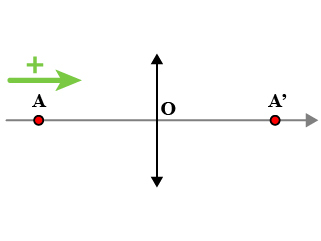
\includegraphics[max size={\textwidth}{0.75\textheight}, center, keepaspectratio]{QCM/Physique/UTC-002/lentille.jpg}
\end{minipage}%
\newline
% Choices
\begin{minipage}[l]{0.45\linewidth}
    \begin{enumerate}
        \item $\overline{OA}$ est positif et $\overline{OA'}$ est négatif.$\overline{OA}$ est positif
        \item $\overline{OA}$ est négatif et $\overline{OA'}$ est positif.$\overline{OA}$ est positif
    \end{enumerate}
\end{minipage}
\hfill
\begin{minipage}[r]{0.45\linewidth}
    \begin{enumerate}
        \item $\overline{OA}$ est positif et $\overline{OA'}$ est négatif.
        \item $\overline{OA}$ est négatif et $\overline{OA'}$ est positif.
    \end{enumerate}    
\end{minipage}

}

%%% QUESTION %%% 
\vspace*{\stretch{1}}
%%% ANSWER %%% 
\color{white}

% Correct answer boxes
\begin{tikzpicture}[remember picture, overlay]
    \node [align=left, opacity=1] at ([xshift = -0.25 cm, yshift = 2.25 cm]current page.center) {
                \color{white}
                \normalsize
                \textsf{\textit{Réponses}}
            };
    \node [align=left, opacity=1] at ([xshift = 2.75 cm, yshift = 2.25 cm]current page.center) {
                \color{white}
                $1:\boxtimes\qquad2:\square\qquad3:\square\qquad4:\square\qquad$\\
                \color{white}
                $5:\square\qquad6:\square\qquad$
            };
\end{tikzpicture}

% Explanations
\vspace{0.05\textheight}
\RaggedRight
Principe d'inertie : Dans un référentiel galiléen, si un système assimilé à un point matériel n'est soumis à aucune force – système isolé – ou s'il est soumis à un ensemble de forces de résultante nulle ($\Sigma\vec{F}_{ext}=\vec{0}$) – système pseudo-isolé – alors il est immobile ou animé d'un mouvement rectiligne uniforme.

Dans cette question, il s'agit de faire la distinction entre mouvement uniforme (la norme de la vitesse est constante, on ne sait rien de la trajectoire) et mouvement rectiligne uniforme ou mouvement circulaire uniforme (norme de la vitesse constante et trajectoire fixée).

%%% ANSWER %%% 
\vspace*{\stretch{1}}
\end{flashcard}

\end{document}